\documentclass[a4paper,10pt]{article}
\usepackage[utf8]{inputenc}

% ----  Useful packages % ---- 
\usepackage{amsmath}
\usepackage{graphicx}
\graphicspath{{images/}}
\usepackage{amsfonts}
\usepackage{amsthm}
\usepackage{amssymb}
\usepackage{makecell}
\usepackage{mathtools}
\usepackage{tikz}
\usepackage{pgfplots}
\usepackage{float}
\usetikzlibrary{arrows.meta}

% ----  Useful packages % ---- 

\usepackage{wrapfig}
\usepackage{caption}
\usepackage{subcaption}
\usepackage{hyperref}
\hypersetup{
	colorlinks,
	citecolor=black,
	filecolor=black,
	linkcolor=black,
	urlcolor=black
}

% ---- Set page size and margins replace ------
\usepackage[letterpaper,top=2cm,bottom=2cm,left=3cm,right=3cm,marginparwidth=1.75cm]{geometry}
% ---- Set page size and margins replace ------

% ------- NOTA ------
\theoremstyle{remark}
\newtheorem{note}{Note}[subsection]
% ------- NOTA ------

% ------- OSSERVAZIONE ------
\theoremstyle{definition}
\newtheorem{observation}{Osservazione}[subsection]
% ------- OSSERVAZIONE ------

% ------- DEFINIZIONE ------
\theoremstyle{plain}
\newtheorem{definition}{Definizione}[subsection]
% ------- DEFINIZIONE ------

% ------- ESEMPIO ------
\theoremstyle{definition}
\newtheorem{example}{Esempio}[subsection]
% ------- ESEMPIO ------

% ------- DIMOSTRAZIONE ------
\theoremstyle{definition}
\newtheorem{demostration}{Dimotrazione}[subsection]
% ------- DIMOSTRAZIONE ------

% ------- TEOREMA ------
\theoremstyle{definition}
\newtheorem{theorem}{Teorema}[subsection]
% ------- TEOREMA ------

% ------- COROLLARIO ------
\theoremstyle{plain}
\newtheorem{corollaries}{Corollario}[theorem]
% ------- COROLLARIO ------

% ------- PROPOSIZIONE ------
\theoremstyle{plain}
\newtheorem{proposition}{Proposizione}[subsection]
% ------- PROPOSIZIONE ------

% ---- Footer and header ---- 
\usepackage{fancyhdr}
\pagestyle{fancy}
\fancyhf{}
\fancyhead[LE,RO]{A.A 2024-2025}
\fancyhead[RE,LO]{Ingegneria del Software}
\fancyfoot[RE,LO]{\rightmark}
\fancyfoot[LE,RO]{\thepage}

\renewcommand{\headrulewidth}{.5pt}
\renewcommand{\footrulewidth}{.5pt}
% ---- Footer and header ---- 

% ----  Language setting ---- 
\usepackage[italian, english]{babel}
% ----  Language setting ---- 

\usepackage{listings}
\usepackage{color}

\definecolor{dkgreen}{rgb}{0,0.6,0}
\definecolor{gray}{rgb}{0.5,0.5,0.5}
\definecolor{mauve}{rgb}{0.58,0,0.82}

\lstset{frame=tb,
	language=C,
	aboveskip=3mm,
	belowskip=3mm,
	showstringspaces=false,
	columns=flexible,
	basicstyle={\small\ttfamily},
	numbers=none,
	numberstyle=\tiny\color{gray},
	keywordstyle=\color{blue},
	commentstyle=\color{dkgreen},
	stringstyle=\color{mauve},
	breaklines=true,
	breakatwhitespace=true,
	tabsize=3
}

\definecolor{lightgray}{rgb}{.9,.9,.9}
\definecolor{darkgray}{rgb}{.4,.4,.4}
\definecolor{purple}{rgb}{0.65, 0.12, 0.82}
\lstdefinelanguage{JavaScript}{
	keywords={break, case, catch, continue, debugger, default, delete, do, else, false, finally, for, function, if, in, instanceof, new, null, return, switch, this, throw, true, try, typeof, var, void, while, with},
	morecomment=[l]{//},
	morecomment=[s]{/*}{*/},
	morestring=[b]',
	morestring=[b]",
	ndkeywords={class, export, boolean, throw, implements, import, this},
	keywordstyle=\color{blue}\bfseries,
	ndkeywordstyle=\color{darkgray}\bfseries,
	identifierstyle=\color{black},
	commentstyle=\color{purple}\ttfamily,
	stringstyle=\color{red}\ttfamily,
	sensitive=true
}

\lstset{
	language=JavaScript,
	extendedchars=true,
	basicstyle=\footnotesize\ttfamily,
	showstringspaces=false,
	showspaces=false,
	tabsize=2,
	breaklines=true,
	showtabs=false,
	captionpos=b
}

\title{\textbf{Ingegneria del software}}
\author{Realizzato da: Ghirardini Filippo}
\date{A.A. 2024-2025}

\begin{document}
	\begin{titlepage} %crea l'enviroment
	\begin{figure}[t] %inserisce le figure
		\centering
\includegraphics[width=0.98\textwidth]{marchio_unipi_pant541.png}
	\end{figure}
	\vspace{20mm}
	
	\begin{Large}
		\begin{center}
			\textbf{Dipartimento di Informatica\\ Corso di Laurea Triennale in Informatica\\}
			\vspace{20mm}
			{\huge{\bf Basi di dati}}\\
			\vspace{5mm}
			{\LARGE{Green City}}\\
			{\large{14 Maggio 2025}}
		\end{center}
	\end{Large}
	
	
	\vspace{36mm}
	\centering{
	\begin{minipage}[t]{0.47\textwidth}
		\centering
		{\large{\bf Autori:}\\ \large{Filippo Ghirardini (654829)}}
	\end{minipage}}
	
\end{titlepage}
	
	\tableofcontents
	\newpage
	\maketitle
	\begin{center}
		\vspace{-20pt}
		\rule{11cm}{.1pt} 
	\end{center}
	% !TeX spellcheck = it_IT
\newpage
\section{Descrizione del dominio}
Un \textbf{concorso} è organizzato da uno o più \textbf{organizzatori}, che devono definire la durata del concorso in giorni, la scadenza per la sottomissione delle opere, la scadenza per la valutazione, il numero massimo di opere che possono essere presentate e la durata massima di ogni opera in minuti. Ogni concorso avrà dei \textbf{generi} consentiti (caratterizzati da un nome e descrizione), delle \textbf{lingue} accettate e dei criteri di partecipazione.\\

Ad ogni concorso un \textbf{regista} (che non può essere l'organizzatore) può presentare dei \textbf{cortometraggi} (fino al massimo indicato dagli organizzatori). Ogni cortometraggio è caratterizzato da un nome, la lingua, il genere, la durata in minuti e una trama.\\

Per ogni concorso gli organizzatori nominano dei \textbf{giudici} che compongono il comitato di valutazione. Ogni cortometraggio \textbf{partecipante} è assegnato a tre giudici, ognuno dei quali uno o più cortometraggi ma tutti di registi diversi. Ogni giudice può nominare un \textbf{giudice esterno} per ogni concorso per la valutazione di uno o più cortometraggi.\\

La valutazione avviene tramite una \textbf{recensione} scritta da un giudice relativamente ad una \textbf{partecipazione} di un cortometraggio, e contiene un punteggio da 0 a 5, un commento generale e una nota riservata.\\

Giudici, organizzatori e registi sono \textbf{utenti} del sistema con nome, cognome, codice fiscale ed email (usata per gli inviti dei giudici).

\newpage
\section{Schema concettuale}
\begin{center}
	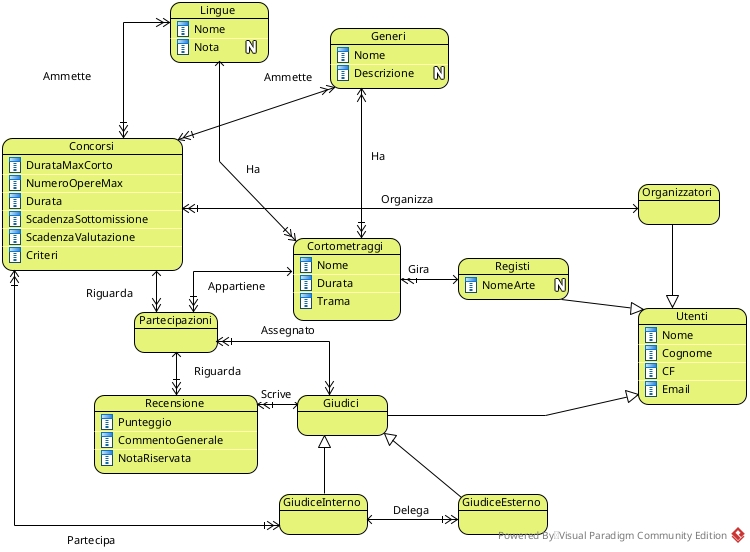
\includegraphics[scale=.5]{ERD_ConCorto.jpg}
\end{center}

\begin{note}
	Al momento della delega da parte di un \textbf{Giudice interno} di un \textbf{Giudice esterno}, quest'ultimo viene inserito nel database e viene assegnato alla valutazione di una determinata \textbf{partecipazione} scelta dal delegante.
\end{note}

\begin{note}
	Al momento dell'inserimento della \textbf{partecipazione} di un \textbf{cortometraggio} ad un \textbf{concorso}, vanno controllati i limiti imposti dall'\textbf{organizzatore} (\textit{DurataMaxCorto}, \textit{NumeroOpereMax}, lingue e generi accettati).
\end{note}

\subsection{Vincoli}
\subsubsection{Interrelazionali}
I vincoli interrelazionali sono:
\begin{itemize}
	\item Un giudice non può giudicare più di un cortometraggio per regista
	\item Un cortometraggio ha 3 giudici assegnati
	\item Un giudice può delegare al più un esterno per ogni concorso
	\item Un organizzatore non può partecipare come regista ad un concorso che organizza
	\item Un giudice può scrivere una sola recensione per cortometraggio per ogni concorso
	\item Se un giudice ha delegato la valutazione non può scrivere la recensione per il cortometraggio che ha delegato
\end{itemize}
\subsubsection{Intrarelazionali}
I vincoli intrarelazionali sono:
\begin{itemize}
	\item \textbf{Generi}: \textit{Descrizione} è NULLABLE
	\item \textbf{Lingue}: \textit{Nota} è NULLABLE
	\item \textbf{Concorsi}: \textit{DurataMaxCorto} $> 0$, \textit{NumeroOpereMax} $>0$, \textit{Durata} $>0$, \textit{ScadenzaSottomissione} $<$ \textit{ScadenzaValutazione}
	\item \textbf{Cortometraggi}: \textit{Durata} $>0$
	\item \textbf{Recensione}: $0\leq$\textit{Punteggio} $\leq 5$
	\item \textbf{Utenti}: \textit{Email} deve rispettare la seguente REGEX
	\begin{lstlisting}[language=Javascript]
		/^[\w-\.]+@([\w-]+\.)+[\w-]{2,4}$/g
	\end{lstlisting}
	\textit{CF} deve rispettare la seguente REGEX
	\begin{lstlisting}[language=Javascript]
		/^(?:[A-Z][AEIOU][AEIOUX]|[AEIOU]X{2}|[B-DF-HJ-NP-TV-Z]{2}[A-Z]){2}(?:[\dLMNP-V]{2}
		(?:[A-EHLMPR-T](?:[04LQ][1-9MNP-V]|[15MR][\dLMNP-V]|[26NS][0-8LMNP-U])|[DHPS]
		[37PT][0L]|[ACELMRT][37PT][01LM]|[AC-EHLMPR-T][26NS][9V])|(?:[02468LNQSU][048LQU]
		|[13579MPRTV][26NS])B[26NS][9V])(?:[A-MZ][1-9MNP-V][\dLMNP-V]{2}|[A-M][0L]
		(?:[1-9MNP-V][\dLMNP-V]|[0L][1-9MNP-V]))[A-Z]$/i
	\end{lstlisting}
	\item \textbf{Registi}: \textit{NomeArte} è NULLABLE
\end{itemize}
Dove non specificato, l'attributo è NON NULLABLE.

\newpage
\section{Schema logico relazionale}
\begin{center}
	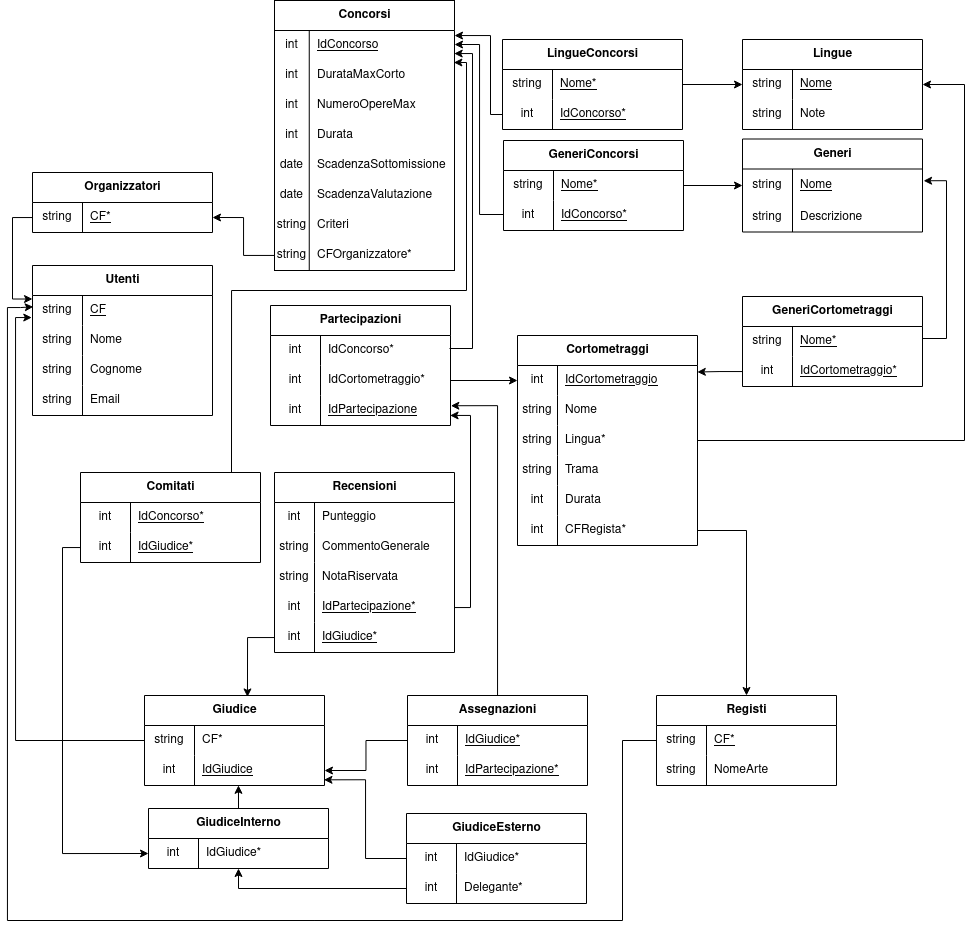
\includegraphics[scale=0.45]{BD0525_logico}
\end{center}

\subsection{Dipendenze funzionali}
Tutte le relazioni $R$ con attributi $A_1, \ldots, A_n$ chiave $K \notin A_1, \ldots, A_n$ hanno una sola dipendenza funzionale del tipo $K \to A_1, \ldots, A_n$.

\subsection{BCNF}
Tutte le relazioni sono in BCNF.

\newpage
\section{Interrogazioni in SQL}
Di seguito le sei interrogazioni richieste:
\begin{enumerate}
	\item[a.] Trova i nomi e le email degli utenti che sono registi e hanno diretto un cortometraggio di durata superiore a 25 minuti.
	\begin{lstlisting}[language=SQL]
		SELECT U.Nome, U.Email
		FROM Utenti U
		JOIN Registi R ON U.CF = R.CF
		JOIN Cortometraggi C ON R.CF = C.CFRegista
		WHERE C.Durata > 25;
	\end{lstlisting}
	\item[b.] Trova i concorsi con più di due lingue ammesse e con una durata massima inferiore a 120 giorni ordinati per numero di lingue in ordine decrescente.
	\begin{lstlisting}[language=SQL]
		SELECT C.IdConcorso, C.Durata, COUNT(L.Nome) AS NumeroLingue
		FROM Concorsi C
		JOIN LingueConcorsi LC ON C.IdConcorso = LC.IdConcorso
		JOIN Lingue L ON L.Nome = LC.Nome
		WHERE C.Durata < 120
		GROUP BY C.IdConcorso, C.Durata
		HAVING COUNT(L.Nome) > 2
		ORDER BY NumeroLingue DESC;
	\end{lstlisting} 
	\item[c.] Trova i generi di cortometraggi lunghi almeno 20 minuti che hanno una durata media superiore a 22 minuti, raggruppati per genere.
	\begin{lstlisting}[language=SQL]
		SELECT G.Nome, AVG(C.Durata) AS DurataMedia
		FROM GeneriCortometraggi GC
		JOIN Generi G ON G.Nome = GC.Nome
		JOIN Cortometraggi C ON C.IdCortometraggio = GC.IdCortometraggio
		WHERE C.Durata > 20
		GROUP BY G.Nome
		HAVING AVG(C.Durata) > 22;
	\end{lstlisting} 
	\item[d.] Trova i nomi dei cortometraggi che hanno almeno una recensione con punteggio superiore a 2.
	\begin{lstlisting}[language=SQL]
		SELECT C.Nome
		FROM Cortometraggi C
		WHERE EXISTS (
			SELECT *
			FROM Recensioni R
			JOIN Partecipazioni P ON R.IdPartecipazione = P.IdPartecipazione
			WHERE P.IdCortometraggio = C.IdCortometraggio AND R.Punteggio > 2
		);
	\end{lstlisting} 
	\item[e.] Trova i nomi dei concorsi in cui tutti i cortometraggi partecipanti hanno una durata inferiore a 30 minuti.
	\begin{lstlisting}[language=SQL]
		SELECT C.IdConcorso
		FROM Concorsi C
		WHERE NOT EXISTS (
		SELECT *
			FROM Partecipazioni P
			JOIN Cortometraggi CM ON P.IdCortometraggio = CM.IdCortometraggio
			WHERE P.IdConcorso = C.IdConcorso AND CM.Durata >= 30
		);
	\end{lstlisting}
	\newpage
	\item[f.] Trova i giudici che hanno assegnato un punteggio superiore alla media dei punteggi di tutti i giudici.
	\begin{lstlisting}[language=SQL]
		SELECT G.IdGiudice, G.CF
		FROM Giudici G
		WHERE EXISTS (
			SELECT *
			FROM Recensioni R
			WHERE R.IdGiudice = G.IdGiudice AND R.Punteggio > (
				SELECT AVG(Punteggio) 
				FROM Recensioni
			)
		);
	\end{lstlisting} 
\end{enumerate}

\newpage
\section{Piani di accesso}
\begin{enumerate}
	\item[I.] Piani di accesso \textbf{logico}
	\begin{figure}[!h]
		\centering
		\begin{minipage}{\textwidth}
			\centering
			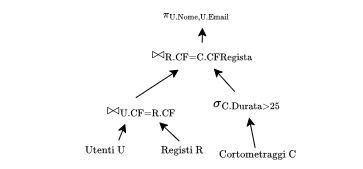
\includegraphics[scale=0.7]{1a.png}
			\captionof{figure}{Query \textit{a}}
		\end{minipage}
		\begin{minipage}{\textwidth}
			\centering
			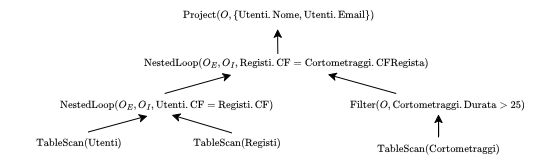
\includegraphics[scale=0.7]{1b.png}
			\captionof{figure}{Query \textit{b}}
		\end{minipage}
		\begin{minipage}{\textwidth}
			\centering
			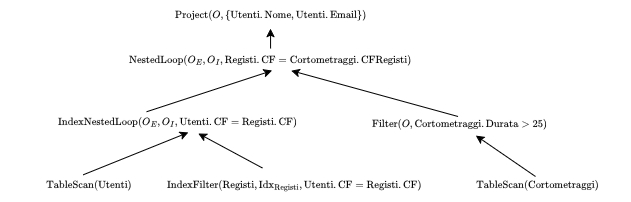
\includegraphics[scale=0.65]{1c.png}
			\captionof{figure}{Query \textit{c}}
		\end{minipage}
	\end{figure}
	
	\newpage
	\item[II.] Piani di accesso \textbf{fisico} senza uso di indici
	\begin{figure}[!h]
		\centering
		\begin{minipage}{\textwidth}
			\centering
			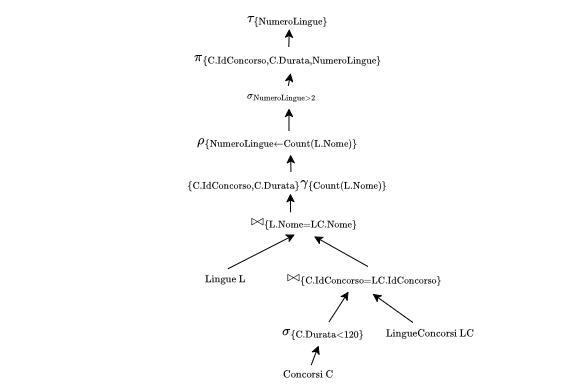
\includegraphics[scale=0.7]{2a.png}
			\captionof{figure}{Query \textit{a}}
		\end{minipage}\\
		\begin{minipage}{\textwidth}
			\centering
			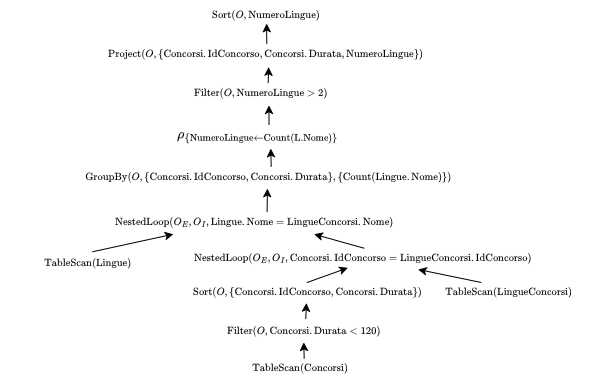
\includegraphics[scale=0.7]{2b.png}
			\captionof{figure}{Query \textit{b}}
		\end{minipage}
	\end{figure}
	\begin{figure}[!h]
		\centering
		\begin{minipage}{\textwidth}
			\centering
			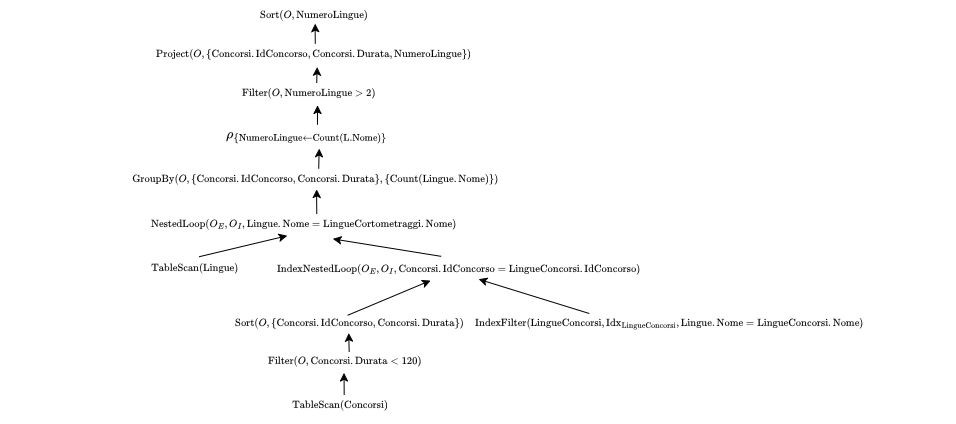
\includegraphics[scale=0.55]{2c.png}
			\captionof{figure}{Query \textit{c}}
		\end{minipage}
	\end{figure}
	
	\newpage
	\item[III.] Piani di accesso \textbf{fisico} con uso di indici
	\begin{figure}[!h]
		\centering
		\begin{minipage}{\textwidth}
			\centering
			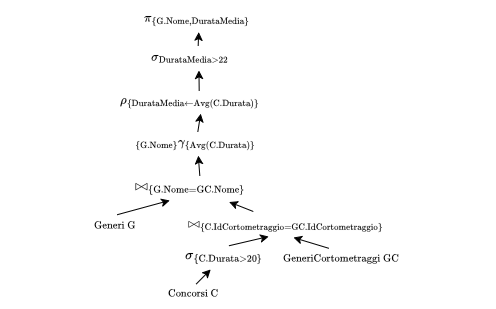
\includegraphics[scale=0.7]{3a.png}
			\captionof{figure}{Query \textit{a}}
		\end{minipage}\\
	\end{figure}
	\begin{figure}[!h]
		\centering
		\begin{minipage}{\textwidth}
			\centering
			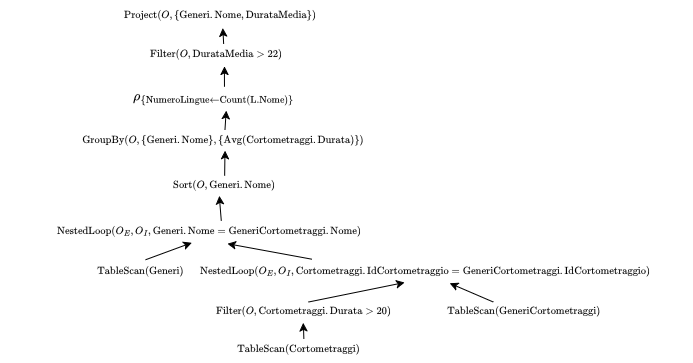
\includegraphics[scale=0.7]{3b.png}
			\captionof{figure}{Query \textit{b}}
		\end{minipage} \hspace{50pt}
		\begin{minipage}{\textwidth}
			\centering
			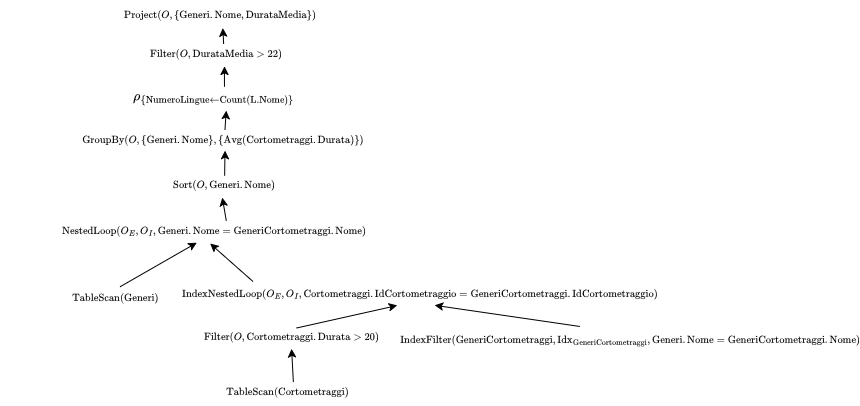
\includegraphics[scale=0.45]{3c.png}
			\captionof{figure}{Query \textit{c}}
		\end{minipage}
	\end{figure}
\end{enumerate}
	\input{softwareprocesses}
	\input{requisiti}
	\input{UML}
	% !TeX spellcheck = it_IT
\newpage
\section{Progettazione}
La fase di progettazione è tra quella della specifica (cosa fare) e quella della programmazione. Come risultato produce un'\textbf{architettura} che descrive \textbf{come} fare.\\
Possono esserci due livelli di astrazione:
\begin{itemize}
	\item \textbf{Architetturale}: si scompone un sistema in più sottosistemi, ne si identificano e specificano le parti e le interconnessioni
	\item Di \textbf{dettaglio}: indica come la specifica di ogni parte sarà realizzata
\end{itemize}

\begin{definition}[Architettura software]
	L’architettura di un sistema software è la \textbf{struttura} del sistema, costituita dalle parti del sistema, dalle \textbf{relazioni} tra le parti e dalle loro proprietà visibili.
\end{definition}

\begin{definition}[Stile architetturale]
	Uno stile architetturale caratterizza una famiglia di architetture con caratteristiche simili (e.g. client-server, microservizi). Le funzionalità e le interazioni tra i componenti spesso seguono degli standard.
\end{definition}

Un'architettura si sviluppa in diverse \textbf{viste} e \textbf{stili}.

\begin{center}
	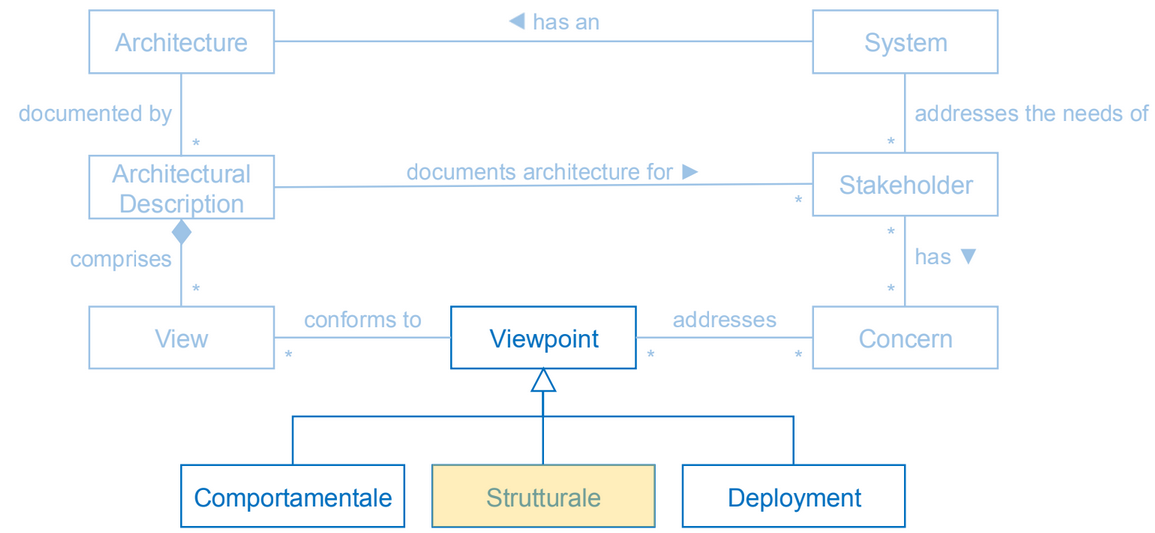
\includegraphics[scale=0.3]{progettazione}
\end{center}

\subsection{Vista comportamentale}
Anche detta \textbf{component-and-connector}, descrive un sistema software come \textbf{composizione di componenti}, compreso di:
\begin{itemize}
	\item \textbf{Interfacce} dei componenti
	\item Caratteristiche dei \textbf{connettori}
	\item Struttura del sistema in esecuzione (flusso dei dati, parallelismo, replicazioni, etc..)
\end{itemize}
Questa vista permette l'analisi delle \textbf{caratteristiche di qualità} a tempo di esecuzione (prestazioni, affidabilità, etc..) e di documentare lo \textbf{stile} dell'architettura.

\subsubsection{Componente}
Una componente software è un'unità concettuale di decomposizione del sistema a tempo di esecuzione. Incapsula un insieme di \textbf{funzionalità} e/o \textbf{dati}, restringendone l'accesso tramite delle \textbf{interfacce}.
\begin{definition}[Componente]
	Una componente software è un'unità di software \textbf{indipendente} e \textbf{riutilizzabile}.
\end{definition}

\begin{definition}[Sistema software]
	Un sistema software è una composizione di componenti software basata sulla connessione di più componenti e realizzata con interfacce dei componenti e connettori,
\end{definition}

\noindent In UML un componente è un \textbf{classificatore} e si compone di:
\paragraph{Porti} I porti ne identificano i punti di interazione. Può essercene più di uno, possono fornire o richiedere una o più \textit{interfacce} e possono avere \textit{nomi} e \textit{molteplicità}.
\begin{center}
	\includegraphics[scale=0.3]{component.png}
\end{center}
I porti possono avere la specifica delle interfacce in due modi:
\begin{itemize}
	\item \textbf{Sintetica}: si indica solo quando è \textit{richiesta} (forchetta) o offerta (\textit{lollipop})
	\begin{center}
		\includegraphics[scale=0.2]{interfaccia_sintetica.png}
	\end{center}
	\item \textbf{Estesa}: si specifica per esteso le operazioni richieste ed offerte
	\begin{center}
		\includegraphics[scale=0.2]{interfaccia_estesa.png}
	\end{center}
\end{itemize}

\paragraph{Connettori}
I connettori sono \textbf{canali di interazione} tra i porti di componenti. Non hanno un descrittore specifico e vengono rappresentati come associazioni. Per dare più informazioni si indica lo \textbf{stile} della connessione o con uno \textbf{stereotipo} o indicando i \textbf{ruoli}.

\begin{center}
	\includegraphics[scale=0.3]{connettori.png}
\end{center}

\subsubsection{Stili}
In questo tipo di vista uno stile architetturale è caratterizzato dalle \textbf{caratteristiche generali} delle componenti e dalle loro \textbf{interazioni} (quindi \textit{porti} e \textit{connettori}).

\paragraph{Pipes \& filters} Questo stile consiste in un flusso di elaborazione di dati che viaggiano lungo le \textbf{pipe} e sono processati dai \textbf{filter}. In particolare i \textit{filter} sono i \textbf{componenti} che trasformano i flussi di dati mentre le \textit{pipe} sono i \textbf{connettori} che fungono da canale di comunicazione unidirezionale bufferizzato che preserva l'ordine di ingresso.
\begin{center}
	\includegraphics[scale=0.3]{pipes_filters.png}
\end{center}

\paragraph{Client-server} Questo stile prevede due componenti che possono essere su macchine diverse. Il \textbf{server} offre il servizio, aspetta le richieste dati ad un porto e può servirne su di esso più alla volta. Il \textbf{client} invia richieste al server e attende una risposta.
\begin{center}
	\includegraphics[scale=0.3]{client-server.png}
\end{center}
Il server in particolare prevede un \textbf{RequestListener} in attesa di richieste e un \textbf{RequestHandler} per ognuna di esse. Quest'ultimo elabora le richieste e:
\begin{itemize}
	\item Se \textbf{stateless} le gestisce ognuna in maniera indipendente
	\item Se \textbf{stateful} consente richieste \textit{composite} che consistono in più richieste \textit{atomiche}, mantenendo un record di esse \textbf{sessione}
\end{itemize}

\paragraph{Master-slave}
Questo stile è una variazione di \textit{client-server} in cui c'è solamente un servente (\textbf{slave}) e un cliente (\textbf{master})

\paragraph{Peer to Peer} Questo stile è una variazione di \textit{client-server} dove tutti i componenti sono sia client che server e avviene uno scambio di servizi alla pari.
\begin{center}
	\includegraphics[scale=0.6]{p2p.png}
\end{center}

\paragraph{Publish-Subscribe} In questo stile i componenti interagiscono in modo \textbf{event-based}. Abbiamo tre tipi di componenti:
\begin{itemize}
	\item \textbf{Publisher}: produce classi di eventi
	\item \textbf{Subscriber}: si iscrive alle classi rilevanti
	\item \textbf{Broker}: smista gli eventi pubblicati
\end{itemize}
Un componente può essere sia \textit{publisher} che \textit{subscriber}. Tra di loro comunicano tramite il \textit{broker}.I publisher non sanno quanti/quali subscriber ci siano e viceversa, garantendo \textbf{scalabilità}.
Questo stile può funzionare in due modi:
\begin{itemize}
	\item \textbf{Push}: il broker invia attivamente i messaggi ai subscriber, controllandone la frequenza
	\item \textbf{Pull}: è il subscriber che manualmente recupera i messaggi dal broker. Migliora la scalabilità e la flessibilità dato che servono meno broker.
\end{itemize}

\begin{figure}[!h]
	\centering
	\begin{minipage}[b]{0.5\textwidth}
		\includegraphics[width=\textwidth]{pub-sub.png}
	\end{minipage}
	\hfill
	\begin{minipage}[b]{0.4\textwidth}
		\includegraphics[width=\textwidth]{pub_sub_full.png}
	\end{minipage}
\end{figure}

\paragraph{Process coordinator}
Un componente funge da \textbf{process coordinator} mentre gli altri sono passivi e non conoscono il loro ruolo nel processo ma si limitano a contribuire. Il \textit{coordinator} conosce la sequenza di passi necessaria, invoca le funzionalità richieste e fornisce una risposta.

\paragraph{Model-View-Controller/Publisher}
Questo stile si basa su tre elementi:
\begin{itemize}
	\item \textbf{Model}: nucleo funzionale che implementa la business logic dell'applicazione e ne rappresenta i dati su cui essa lavora
	\item \textbf{View}: presentazione del model all'utente, possono essercene diverse
	\item \textbf{Controller}: controlla l'input dell'utente e lo traduce in operazioni da eseguire su \textit{model} oppure \textbf{presenter} in alternativa
\end{itemize}
\begin{figure}[!h]
	\centering
	\begin{minipage}[b]{0.4\textwidth}
		\includegraphics[width=\textwidth]{model_view_controller.png}
		\caption*{Controller}
	\end{minipage}
	\hspace{10pt}
	\begin{minipage}[b]{0.4\textwidth}
		\includegraphics[width=\textwidth]{model_view_presenter.png}
		\caption*{Presenter}
	\end{minipage}
\end{figure}

\subsection{Vista strutturale}
Descrive la struttura di un sistema software come insieme di \textbf{unità di realizzazione}, ovvero di codice. Permette di analizzare le \textbf{dipendenze}, progettare i \textbf{test} e valutare la \textbf{portabilità}.\\
La vista strutturale in UML include:
\begin{itemize}
	\item \textbf{Classi} con specifica delle \textit{operazioni} più dettagliata rispetto alla descrizione del dominio
	\item \textbf{Package}
\end{itemize}

\subsubsection{Decomposizione}
\begin{wrapfigure}[7]{r}{5cm}
	\vspace{-1.2cm}
	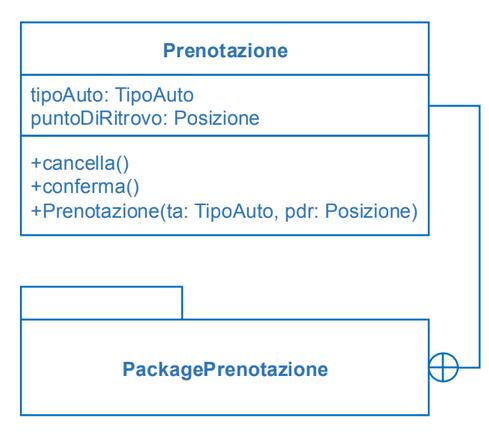
\includegraphics[width=5cm]{decomposizione}
\end{wrapfigure}
Una classe può far parte (essere contenuta in) un package, che a sua volta può far parte di uno più grande. La decomposizione può essere fatta per \textbf{apprendimento} del sistema o per l'\textbf{allocazione del lavoro} e può seguire tre criteri:
\begin{itemize}
	\item Incapsulamento per \textbf{modificabilità}
	\item Supporto alle scelte \textbf{costruisci}/\textbf{compra}
	\item Moduli comuni in \textbf{linee di prodotto}
\end{itemize}

\begin{note}
	La relazione "parte di" si può rappresentare anche con l'inclusione grafica in un package.
\end{note}

\newpage

\subsubsection{Uso}
Un modulo A può usarne un altro B per soddisfare i suoi requisiti. Questo permette di pianificare uno sviluppo incrementale e creare test di unità ed integrazione. Sono permessi i cicli anche se pericolosi.

\begin{center}
	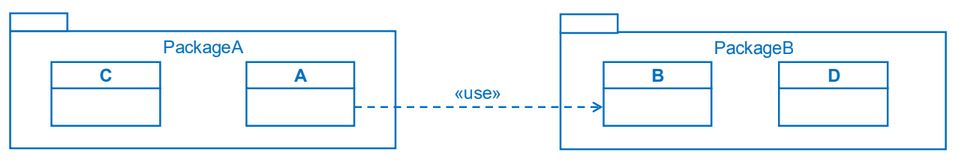
\includegraphics[scale=0.4]{uso}
\end{center}

\subsubsection{Strati}
\begin{wrapfigure}[10]{r}{3cm}
	\vspace{-1cm}
	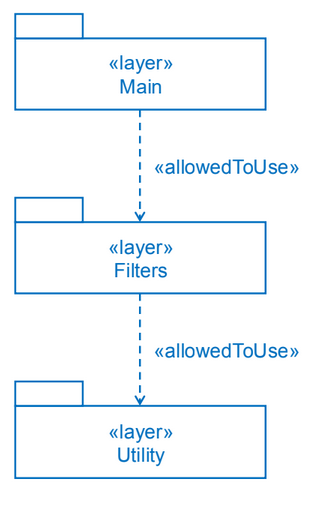
\includegraphics[width=3cm]{strati}
\end{wrapfigure}
Nella vista strutturale a strati ogni elemento (\textbf{strato}) è un insieme coeso di moduli a volte raggruppati in segmenti, il quale offre un'interfaccia pubblica per i suoi servizi. La relazione \textit{allowedToUse} è un caso particolare di quella di uso ed è \textbf{antisimmetrica} e \textbf{non implicitamente transitiva}.\\
Questa vista favorisce modificabilità, portabilità e controllo della complessità.

\subsubsection{Generalizzazione}
In questa vista gli elementi sono i \textbf{moduli} (classi o packages) che hanno una relazione di generalizzazione tra di loro. Permette di rappresentare relazioni di sotto tipo tra classi e la relazione tra un framework\footnote{Collezione di classi, anche astratte, con relazioni d'uso tra loro.} e una sua specializzazione nel caso dei package.

\subsection{Vista di deployment}
Descrive l'allocazione del software su ambienti di esecuzione e permette di valutarne \textbf{prestazioni} e \textbf{affidabilità}. Contiene:
\begin{itemize}
	\item \textbf{Artefatti} prodotti da un processo di sviluppo software o dal funzionamento di un sistema, rappresentati dallo stereotipo \textit{$<<$artifact$>>$}
	\item \textbf{Ambienti di esecuzione} o nodi hardware, rappresentati come \textit{parallelepipedi}
\end{itemize}
Questi elementi possono avere due tipi di relazioni:
\begin{itemize}
	\item \textbf{Dislocazione} di artefatti negli ambienti, rappresentata con il \textit{contenimento}
	\item \textbf{Interconnessione} tra gli ambienti di esecuzione, rappresentate con relazioni stereotipate
\end{itemize}
\begin{center}
	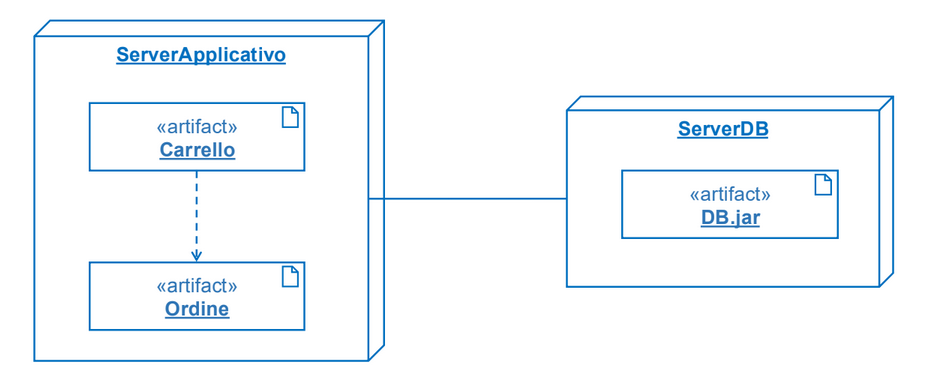
\includegraphics[scale=.4]{deployment}
\end{center}

\subsection{Vista ibrida}
La vista ibrida si compone di quella comportamentale e di quella di deployment su di un'applicazione 3-tier.
\begin{center}
	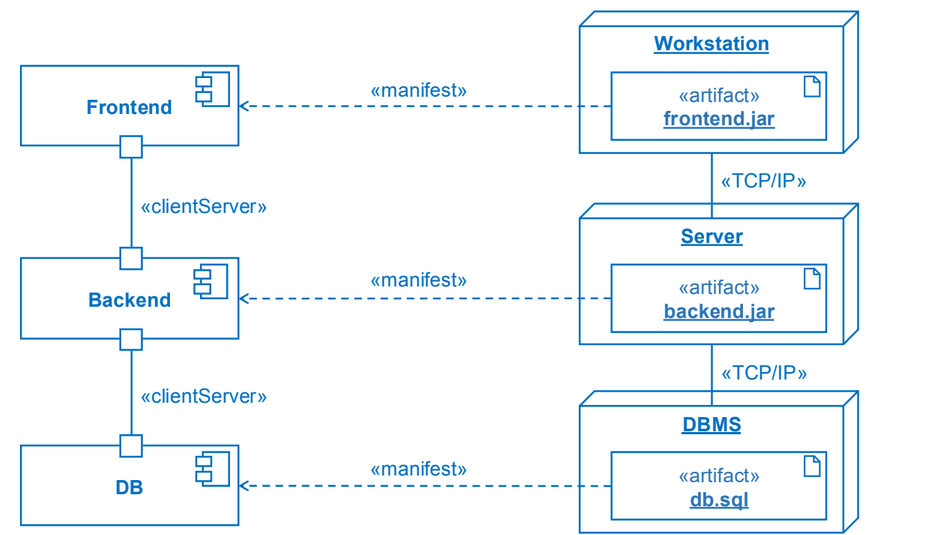
\includegraphics[scale=.4]{ibride}
\end{center}

\subsection{Altri esempi}
\subsubsection{Architettura a livelli}
\begin{wrapfigure}[9]{r}{6cm}
	\vspace{-1cm}
	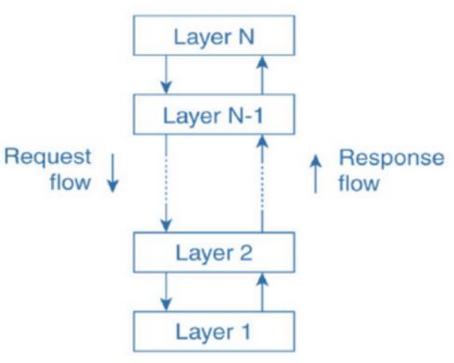
\includegraphics[width=6cm]{livelli}
\end{wrapfigure}
I componenti sono organizzati in livelli (layer) dove uno a livello $i$ può invocarne uno del livello sottostante $i-1$. Le richieste scendono lungo la gerarchia mentre le risposte salgono.

\subsubsection{Architettura multi-livello}
In questa architettura avviene un mapping tra livelli logici (layer) e fisici (tier). Può avere da $1$ ad $N$ livelli, dove all'aumentare di questi si guadagna in \textbf{flessibilità}, \textbf{funzionalità} e possibilità di \textbf{distribuzione} ma si introducono problemi di \textbf{prestazione}. \\
Dal punto di vista fisico, l'architettura può essere:
\begin{itemize}
	\item \textbf{1-tier}: mainframe e terminale
	\item \textbf{2-tier}: macchina client e singolo server
	\item \textbf{3-tier}: ciascun livello su una macchina separate
\end{itemize}
\begin{center}
	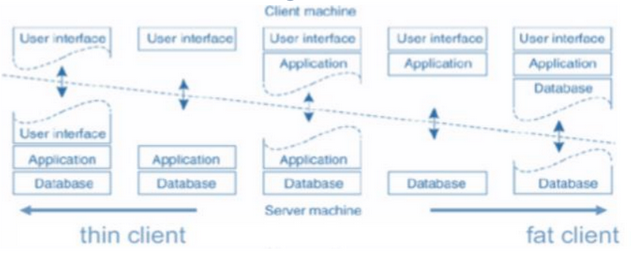
\includegraphics[scale=.4]{multiliv}
\end{center}
	% !TeX spellcheck = it_IT
\newpage
\section{Diagrammi di sequenza}
\begin{wrapfigure}[10]{r}{5cm}
	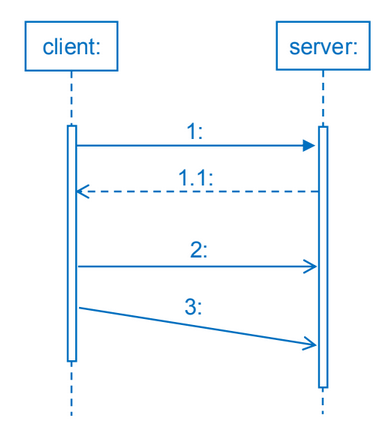
\includegraphics[width=5cm]{diagseq}
\end{wrapfigure}
I diagrammi di sequenza descrivono le \textbf{interazioni} tra oggetti riorganizzandole in una sequenza temporale. Nella fase di \textit{analisi} dei casi d'uso formalizzano la sequenza principale  degli eventi mentre in fase di \textit{progettazione} illustrano come l'architettura realizza i requisiti.\\

In UML per ogni partecipante viene disegnata una \textbf{linea di vita} che può essere tratteggiata quando l'oggetto è inattivo e doppia-continua quando è attivo. Per rappresentare le \textbf{interazioni} vengono usate frecce, che possono essere:
\begin{itemize}
	\item \textbf{Sincrone}
	\item \textbf{Ritorno}
	\item \textbf{Asincrone}
	\item Asincrone con \textbf{consumo di tempo}
\end{itemize}

\subsection{Etichette}
È possibile mettere etichette ai messaggi:
\begin{itemize}
	\item $n$ è il numero del messaggio nella sequenza
	\item \textbf{attr} è l'attributo a cui assegnare il valore restituito
	\item \textbf{name} identifica e descrive il messaggio
	\item \textbf{arg} sono i parametri
	\item \textbf{value} rappresenta il valore restituito
\end{itemize}
\begin{center}
	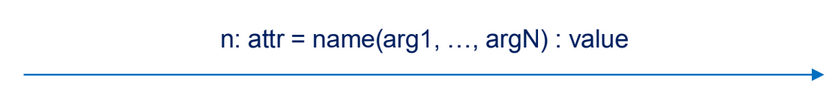
\includegraphics[scale=.4]{etichette}
\end{center}

\subsection{Creazione e distruzione}
Un oggetto può crearne o eliminarne un altro attraverso lo scambio di messaggi.
\begin{center}
	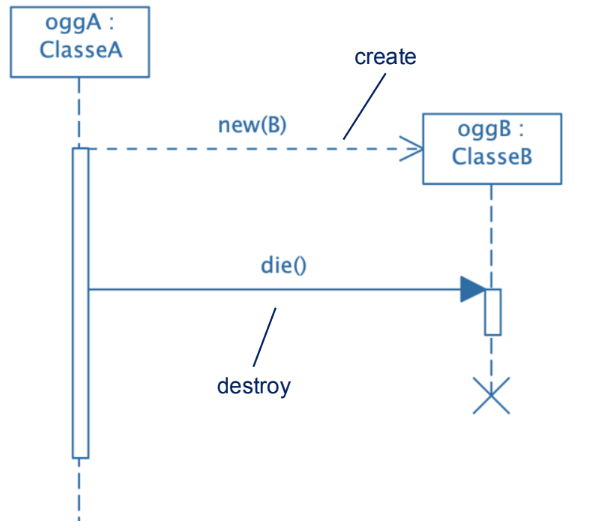
\includegraphics[scale=0.4]{creazdist}
\end{center}

\subsection{Frame}
\subsubsection{Condizionale}
È identificato dalla parola \textbf{alt}. I subframe possono essere etichettati con guardie:
\begin{itemize}
	\item Se non c'è la guardia, è \textit{true}
	\item Se ci sono più guardie vere è una situazione di non determinismo
	\item Se ci sono tutte le guardie false, si salta il frame
\end{itemize}
\begin{center}
	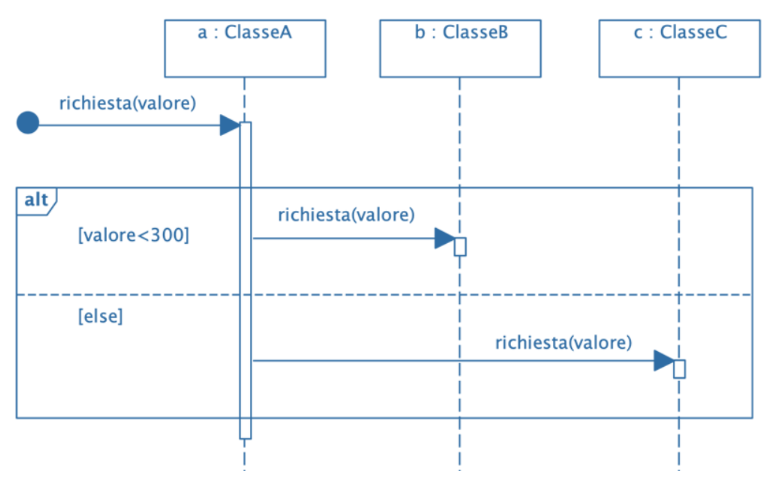
\includegraphics[scale=.3]{condiz}
\end{center}

\subsubsection{Opzionale}
Il frame opzionale è identificato dalla parola chiave \textbf{opt} e le interazioni sono eseguite solo se la guardia è vera, altrimenti il frame viene saltato.
\begin{center}
	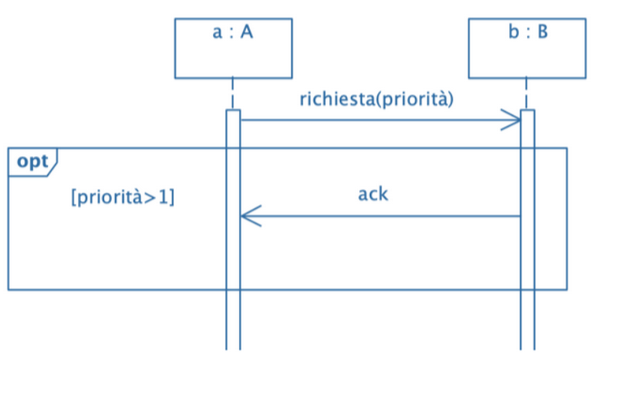
\includegraphics[scale=.3]{opz}
\end{center}

\subsubsection{Iterativo}
Questo frame ripete il suo contenuto da \textit{min} a \textit{max}, \textbf{loop(min, max)} e finché la \textbf{condizione} è vera. Quindi le implementazioni dei classici cicli sono:
\begin{itemize}
	\item \textbf{while}: loop(0,*)[guardia] e loop[guardia]
	\item \textbf{do-while}: loop(1,*)[guardia]
	\item \textbf{for}: loop(n,n) e loop(n)
\end{itemize}
\begin{center}
	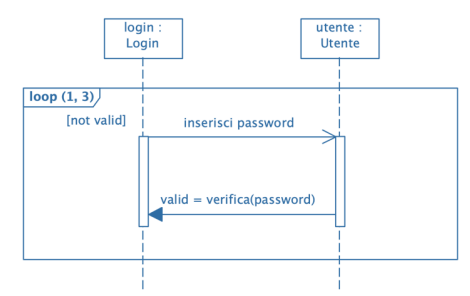
\includegraphics[scale=.4]{cicli}
\end{center}

\subsubsection{Parallelo}
Identificato da \textbf{par}, indica che le interazioni nei sotto-frammenti sono eseguite in parallelo con una semantica ad interleaving.

\begin{center}
	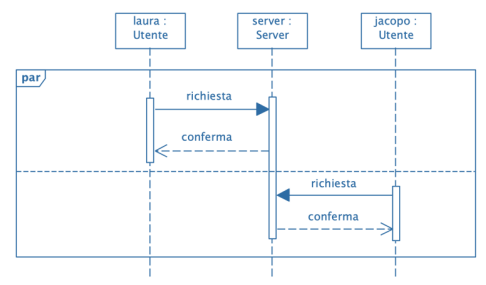
\includegraphics[scale=.5]{parall}
\end{center}

\subsection{Inclusione}
È possibile includere un'interazione definita altrove tramite \textbf{ref}.
\begin{center}
	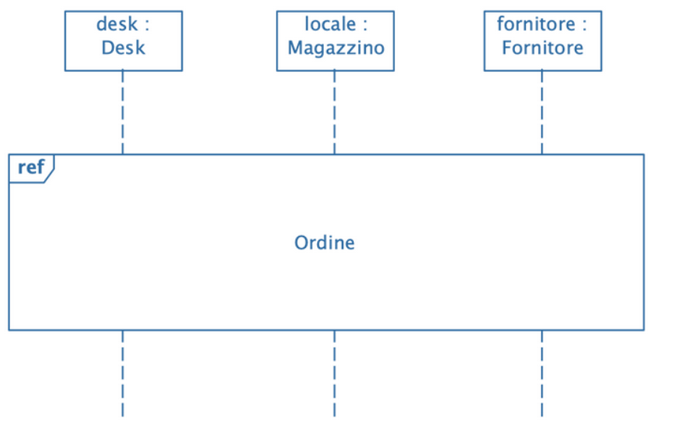
\includegraphics[scale=.4]{ref}
\end{center}

\subsection{Gate}
Un gate è un punto di ingresso o di uscita sul bordo di un diagramma o di un frame. Consente la spedizione e la ricezione di messaggi ed è identificato da un nome.
\begin{center}
	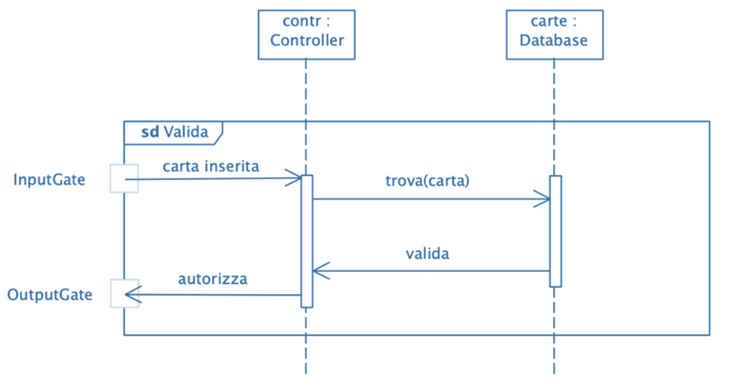
\includegraphics[scale=.4]{gate}
\end{center}

\subsection{Vincoli di durata}
Sono espressi tra parentesi graffe e consentono di specificare:
\begin{itemize}
	\item \textbf{quando} avviene un evento, tramite \textbf{at}(orario) o \textbf{now}
	\item \textbf{quanto} tempo tra due eventi, che può essere un numero effettivo o un range (min, max)
\end{itemize}
\begin{center}
	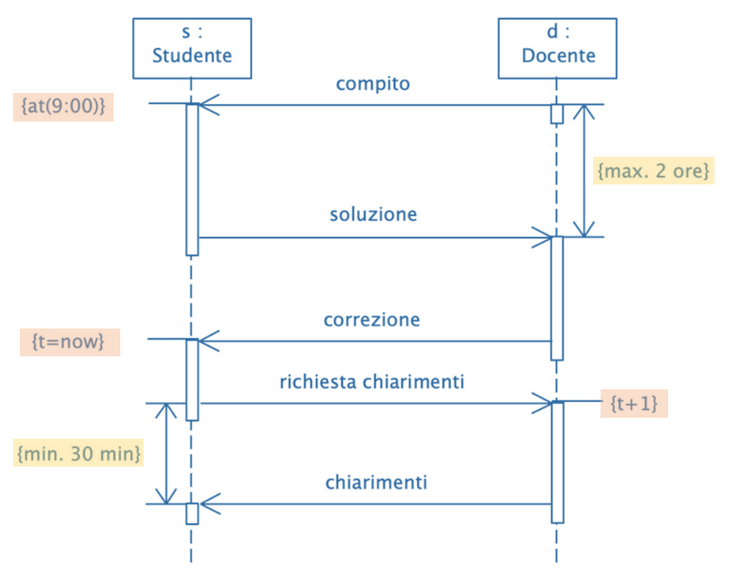
\includegraphics[scale=.4]{vincoli}
\end{center}
\end{document}
